\documentclass[12pt]{article}

% TEMPLATE DEFAULT PACKAGES
\usepackage{amssymb,amsmath,amsfonts,eurosym,geometry,ulem,graphicx,color,setspace,sectsty,comment,natbib,pdflscape,array,adjustbox}

% ADDED PACKAGES FOR THIS MANUSCRIPT
\usepackage{palatino,newtxmath,multirow,titlesec,threeparttable,tabu,booktabs,titlesec,threeparttable,mathtools,bm,bbm,subcaption,pdflscape,tcolorbox,mathrsfs}
% endfloat,

\usepackage{afterpage}
\usepackage[hyphens]{url}
\usepackage[margin=1cm]{caption}

\usepackage[draft]{hyperref}
\newcommand{\tim}{$\,\times\,$}
% FIGURES & TABLES CAPTION STYLING
\captionsetup[figure]{labelfont={bf},name={Figure},labelsep=period}
\captionsetup[table]{labelfont={bf},name={Table},labelsep=period}

% SECTION TITLE SETTINGS
\titlelabel{\thetitle.\enskip}
\titleformat*{\section}{\large\bfseries}
\titleformat*{\subsection}{\normalsize\bfseries}

% COLUMN TYPES
\newcolumntype{L}[1]{>{\raggedright\let\newline\\\arraybackslash\hspace{0pt}}m{#1}}
\newcolumntype{C}{>{\centering\arraybackslash}p{5.2em}}
\newcolumntype{D}{>{\centering\arraybackslash}p{5em}}
\newcolumntype{R}[1]{>{\raggedleft\let\newline\\\arraybackslash\hspace{0pt}}m{#1}}


% MARGINS AND SPACING
\normalem
\geometry{left=1.1in,right=1.1in,top=1.0in,bottom=1.0in}
\setlength{\parskip}{2.5pt}

% SPECIAL CELL 
\newcommand{\specialcell}[2][c]{%
	\begin{tabular}[#1]{@{}l@{}}#2\end{tabular}}

% NO INDENT ON FOOTNOTES
\usepackage[hang,flushmargin]{footmisc}

\begin{document}

\begin{titlepage} 
\title{{Paying bills}\thanks{We are grateful to Andrew Foster}}
\author{\\[3em]
  William Violette\thanks{Federal Trade Commission, Washington, DC. E-mail: william.j.violette@gmail.com} \\
 \\ 
  }
\vspace{30mm}
\date{\vspace{5mm}This Version: \today}
\maketitle
\begin{abstract}

	paying bills

 %\\

%\vspace{0in}\\
%\textbf{Keywords:} traffic externalities; street livability; urban policy; housing market.\\
%\vspace{0in}\\
%\textbf{JEL Codes:} O18; H4; R2; R4.\\
\bigskip
\end{abstract}
\setcounter{page}{0}
\thispagestyle{empty}
\end{titlepage}
\pagebreak \newpage

\spacing{1}


\section{Pitch}

This paper looks at whether utilities in developing countries provide an important source of credit to households by letting them not pay their bill?  And how do these benefits compare to the costs of delinquency?

Motivation : (1) around the world, there are restrictions on when utilities can disconnect people (health, low-income, elderly), motivated by providing a sense of insurance;  (2) Also, in developing countries, pre-paid metering where utilities essentially put fancy meters that only distribute water when people pay first.  these shut off any credit channel but eliminate delinquency

Context : In Manila, water bills make up about 3\% of income on average, jumps to 5 to 10\% for low-income folks.  I have data from a large water provider serving half the city of Manila.  On average, people make a payment in three out of four months and are about a month behind in payments.  For example, if you don't pay for three months, that's like taking a three-month loan of around 9\% of your income.  

People might be paying infrequently because they are credit-constrained and consumption smoothing; or it might just be a pain to pay their bills so they just avoid the hassle by paying infrequently (and they have plenty of other opportunities to smooth).  

I use disconnection threats to better isolate the role of credit constraints.  Workers will occasionally visit delinquent customers and say if you don't pay your bill soon (within 12 days on average), we'll disconnect you.  Only 23\% of people say that's ``enough time'' to pay the bill.  After the threats, payments spike to double the average bill, delinquency drops to zero, and consumption drops by around 25\%.  If it were simply a hassle, people would pay their bill and consumption wouldn't change (they could get easy credit from other places and pay the bill); but if they are credit constrained, they have to deviate from consumption smoothing to make the payments.  The next step is to use theory to see what this decrease in consumption implies about the short-term interest rate that households face.


\section{Introduction}

%% disconnection 

% https://liheapch.acf.hhs.gov/Disconnect/disconnect.htm
\subsection{Question} 
Are utilities providing an important source of credit to households by letting them not pay their bill?

\subsection{Motivation}
\begin{itemize}
\item Disconnection policies as insurance (in the US) 
	\begin{itemize}
		\item weather, health, low-income
		\item mandate that utilities amortize arrears
		\item Utilities even tolerate greater non-payment
	\end{itemize}
\item At the same time, pre-paid metering is growing like crazy in the developing world (Sources)
\end{itemize}

\subsection{Descriptives}
% How much credit could households get from their water bill?
\begin{itemize}
\item Avg Income: 22,000 PhP (488 USD)   [ Bill 3\% ]
\item Avg Savings: 4,300 PhP (96 USD) 
\item 20\% Income: 8,300 PhP (184 USD)  [ Bill 7.6\% ]
\item 20\% Savings: 330 PhP (7 USD)  
\item Avg Bill: 630 PhP (14 USD)
\item Make payments 75\% of months
\item Avg delinquency: 30 days
\item Avg Payment Amount: 830 PhP (18 USD)
\end{itemize}

But : might just be inconvenient to pay every month (but its really easy to pay bills in this context)

How can I ballpark this against the consumption smoothing literature?

\subsection{Approach}

Disconnection : Don't pay bill; come and threaten disconnection
\begin{itemize}
\item avg days to pay : 12 days (only 23\% say that's enough time)
\item if you (agree to?) pay, you are reconnected after 2 days
\item 30\% of connections are threatened with disconnection
\item (small percent actually disconnect)
\item Pay (+1) 800 PhP (+2) 300 PhP = total 1100 PhP (24 USD) [ about two water bills on average ]
\item Consumption drops by about 20\% for two months (there is a pre-trend which can be interpreted as positive demand shocks)
\end{itemize}

\noindent Theory :
\begin{itemize}
\item suddenly this source of credit is cut off (loan with uncertain payback date)
\item concave utility predicts that households would want to smooth consumption (could get another loan, then fund consumption in that period)
\item 
\end{itemize}


\section{Data}

To measure water consumption and payments, I partnered with a large water provider in Manila who shared administrative data on over 1.5 million water connections.  These data include water consumption and payment data as well as disconnection status.  

Describe notice of disconnection in more detail here???

used to measure water consumption and payment data comes from monthly administrative data from a large water provider in Metro Manila

The 2015 Family Income and Expenditure Survey provides household income measures, which help to calibrate the structural model.  

STICK WITH ONE HOUSEHOLD PER METER IN THIS PAPER!  EXPLAIN THIS IN THE DATA SECTION!  CONNECT TO FIES DATA AS WELL!!


\section{Credit through Unpaid Water Bills}

% \footnote{The company upgraded t in the first year of the sample.  Previously, the company mailed the bill to each household at the end of the month.} 
% Each month, households consume 24m3 of piped water on average, which totals an average monthly bill of 691.6PhP as shown in Table~\ref{table:descriptives_all}.  Given an average monthly income in Manila of 31,910PhP and savings rate of 5,730PhP,  monthly water bills reach a modest average of 2.2\unskip\% of income and 10.6\unskip\% of savings.  


\begin{table}[h!] % PUT IN DEMOGRAPHICS PLEASE ?!?!?
\centering
\caption{Mean Characteristics}\label{table:descriptives_all}
\vspace{-2mm}
\begin{tabular}{l*{1}{cccccc}}
\toprule
 & Mean & SD & Min & 25th & 75th & Max  \\
\midrule
 Usage (m3)  & 24.9  & 17.0  & 0.0  & 14.0  & 32.0  & 200.0  \\ 
 Bill  & 692  & 927  & -4,640  & 265  & 854  & 78,409  \\ 
 Unpaid Balance  & 1,523  & 4,611  & -4,995  & 0  & 1,126  & 79,904  \\ 
 Share of Months with Payment  & 0.71  & 0.45  & 0.00  & 0.00  & 1.00  & 1.00  \\ 
 Payment Size  & 924  & 1,147  & 0  & 316  & 1,082  & 62,879  \\ 
 Days Delinquent  & 50.2  & 133.6  & 0.0  & 0.0  & 31.0  & 720.0  \\ 
 Delinquency Visits per HH  & 0.42  & 0.71  & 0.00  & 0.00  & 1.00  & 6.00  \\ 
 Share of Months Disconnected  & 0.04  & 0.19  & 0.00  & 0.00  & 0.00  & 1.00  \\ 

\bottomrule \\ [-.8em]
\multicolumn{7}{c}{Total Households: 46,098  Obs. per Household: 60.9 Total Obs.: 2,123,335}
\end{tabular}
\end{table}

Unpaid water bills may provide a reliable source of low-cost credit to households because (1) the company tolerates high rates of delinquency before disconnecting them from service and (2) the water company is prohibited from charging any interest on outstanding balances. 

At the end of each month, the water company sends meter readers who record monthly consumption for each connection and then use a mobile device to print and deliver the bill to the household in person.  The household is then expected to pay the bill by the end of the month.  Households have many options to pay their bills with 79\unskip\% using small payment centers (mall kiosks, gas stations, convenient stores, etc.), 9.4\unskip\% paying at local water company offices, and 3\unskip\% paying over phone, online, or via ATM kiosks.\footnote{Figures are tabulated from the connection survey sample.}  Despite easy payment mechanisms, households rarely pay their bills on time.  Table~\ref{table:descriptives_all} provides summary statistics on the usage, billing, and payment patterns of households.  On average, households are 50days behind in their payments.  Households also make large, infrequent payments.  While the average bill is 691.6PhP per month, payment sizes average 901PhP and households make payments in only 61\unskip\% of months.  These payment patterns leave an average total outstanding balance of 2,068PhP per month.  

Given average monthly household incomes of 31,910PhP and savings rates of 5,730PhP in Manila, unpaid water bills reach 4.3\unskip\% of income and 28.7\unskip\% of savings on average each month.  For households at the 20th income percentile, unpaid water bills jump to 10\unskip\% of monthly income.  As a benchmark, \cite{cull2009microfinance} survey microfinance institutions throughout the developing world and find median yearly loan sizes expressed as a share of the 20th percentile of household income at 48\% for nongovernmental organizations (NGOs), 160\% for nonbank financial institutions, and 224\% for banks.  These descriptives suggest that a yearly loan from an NGO could be reached with around 5 months of unpaid water bills for households at the 20th income percentile.\footnote{Deal with income effects on water consumption!}  Moreover, microfinance loans charge high yearly interest ranging from 25\% for NGOs to 13\% for banks.  In comparison, unpaid water bills are interest-free, but households face some risk of service disconnection for delinquency.

After bills have remained unpaid for at least 60 days, the government regulator permits the water company to visit delinquent households to disconnect their water service.\footnote{Regulations also require the water company to issue written statements to households, notifying them that their connections will be disconnected in 7 days if their outstanding balances remain unpaid.  In practice, only 36\unskip\% of disconnected households report receiving advanced notice.  All percentages are calculated from 924respondents who report being visited for disconnection in the past year out of 34,406total respondents in the connection survey.}  Likely due to time and travel costs, delinquency visits are relatively rare in practice, occurring in only 0.70\unskip\% of household-month observations.  This probability increases to 2.90\unskip\% for household-months over 60 days overdue.  Figure~\ref{figure:dc_hazard} plots the share of months with delinquency visits according to days overdue.  The risk of delinquency visits spikes at 61 days overdue before settling to around 2.5\% at higher levels of delinquency.  Appendix Table~\ref{table:tcd_predict} predicts delinquency visits with days overdue, outstanding balance, and household characteristics.  This exercise finds that days overdue and unpaid balances are strongly and independently correlated with visits while demographic indicators have weaker associations. % more to say here about magnitudes?!

When company staff conduct delinquency visits, households often negotiate for additional time to pay their outstanding balances.  96\unskip\% of households report agreeing to pay within 30 days and the average grace period is 13days; however, only 25\unskip\% of connections report having ``enough time'' to make their payments.  For households who fail to pay, disconnection typically involves workers from the water company placing a metal lock on the water meter stopping the flow.  In order to reconnect, households must pay a small, one-time fee of 200 PhP on top of settling any outstanding balances.  The water company is then required to restore service within 48 hours of receiving full payment for reconnection, which is confirmed in survey data.\footnote{Households report being reconnected 2.3days after payment.}  


\begin{figure}
\centering
\caption{Share of Households that Receive a Delinquency Visit \\ depending on Days Delinquent in the Previous Month}\label{figure:dc_hazard}
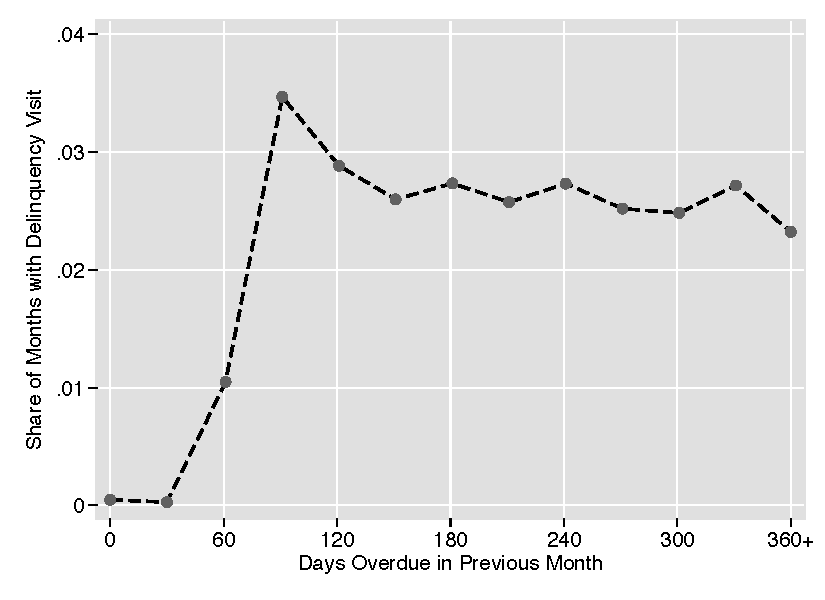
\includegraphics[scale=.7]{tables/connected_visit_hazard_all.pdf}
\end{figure}




\begin{table}[h!]
\centering
\caption{Mean Characteristics by Delinquency Visit Status}\label{table:descriptives_3g}
\vspace{-2mm}
\begin{tabular}{l*{1}{ccc}}
\toprule
 & Never Visited & Stayers & Leavers  \\
% &   &         &        \\
\midrule
 Usage (m3)  & 24.3  & 26.2  & 26.3  \\ 
 Bill  & 658  & 761  & 833  \\ 
 Unpaid Balance  & 706  & 2,416  & 6,520  \\ 
 Share of Months with Payment  & 0.78  & 0.60  & 0.38  \\ 
 Payment Size  & 829  & 1,214  & 1,247  \\ 
 Days Delinquent  & 18.9  & 84.9  & 236.5  \\ 
 Delinquency Visits per HH  & 0.00  & 1.32  & 1.42  \\ 
 Months Disconnected  & 0.01  & 0.03  & 0.31  \\ 
 HH Size  & 5.2  & 5.6  & 5.7  \\ 
 Age of HoH  & 47.4  & 44.8  & 45.8  \\ 
 Low Skilled HoH  & 0.14  & 0.17  & 0.19  \\ 
 &  &  &  \\ 
 Total Households   & 23,727  & 8,260  & 2,419  \\ 
 Total Observations  & 1,464,945  & 509,959  & 148,431  \\ 

\bottomrule
\multicolumn{4}{l}{\scriptsize ``Never Visited'' includes HHs that never receive a delinquency visit.}\\  [-.5em]
\multicolumn{4}{l}{\scriptsize ``Stayers'' includes HHs with $\geq$1 visit and are connected for the last 6 months.}\\ [-.5em]
\multicolumn{4}{l}{\scriptsize ``Leavers'' includes HHs with $\geq$1 visit and are disconnected for $\geq$1 of the last 6 months.}\\ [-.5em]
\multicolumn{4}{l}{\scriptsize Bill, Unpaid Balance, and Payment Size are in PhP/month.} 
\end{tabular}
\end{table}


Table~\ref{table:descriptives_3g} provides mean characteristics according to whether and how households respond to delinquency visits over the course of the sample.  The first column, ``Never Visited,'' includes households that never receive a delinquency visit.  Since delinquency visits are relatively rare, the majority of observations fall into this category.  The second and third columns include households that receive at least one delinquency visit.   The second column, ``Stayers,'' also requires that households are connected for the final 6 months of the sample while the third column, ``Leavers,'' includes households that are disconnected for at least one of the final 6 months of the sample.  

Leavers are predominantly composed of households that permanently disconnect over the sample period, which likely occurs when households move out of their current residences.  These households often leave large outstanding balances that are almost never repaid due to difficulties tracking households across locations.  By incentivizing households to pay, frequent delinquency visits provide a strategy for the company to minimize this lost revenue.

Stayers include households that remain connected at the end of the sample despite receiving at least one delinquency visit over the duration.\footnote{Stayers also excludes 67households that the company has flagged as ``permanently disconnected.''}  Compared to households that are never visited, stayers have much higher outstanding balances and days delinquent.  Their payments also occur less frequently but have larger average sizes.  Stayers spend 3\% of the sample period disconnected from service.  Until they are able to pay for reconnection, these households likely substitute to alternative water sources including sharing with neighbors, using from deepwells, or purchasing from local water vendors.\footnote{Table~\ref{table:descriptives_3g} indicates that even for households that are never visited, they are disconnected during 1\% of months.  These disconnections include (1) households that received a delinquency visit before the start of the sample (but later reconnected) and (2) households that notify the water company about their moving plans in advance and therefore, do not need a delinquency visit.}  Stayers also have slightly larger household sizes, younger heads of household, and greater incidence of low-skilled employment than never visited households.  These demographic patterns are consistent with lower-income households having greater difficulty paying their bills promptly.




\begin{figure*}[t!]
    \centering
    \vspace{2mm}
    \begin{subfigure}[b]{0.49\textwidth}
        \centering
        \caption[]{\small Share Disconnected}  
        \vspace{-1mm}
        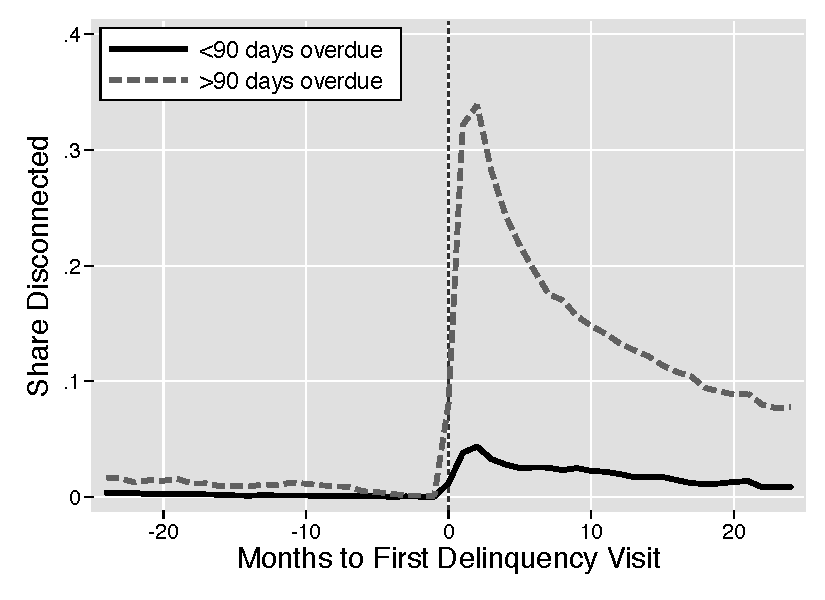
\includegraphics[width=\textwidth,trim={.2cm .2cm .2cm 0cm}, clip=true]{tables/line_disconnection}
        \label{fig:line_disc}
    \end{subfigure}
    \hfill
    \begin{subfigure}[b]{0.49\textwidth}  
        \centering 
        \caption[]{\small Unpaid Balance}
        \vspace{-1mm}
        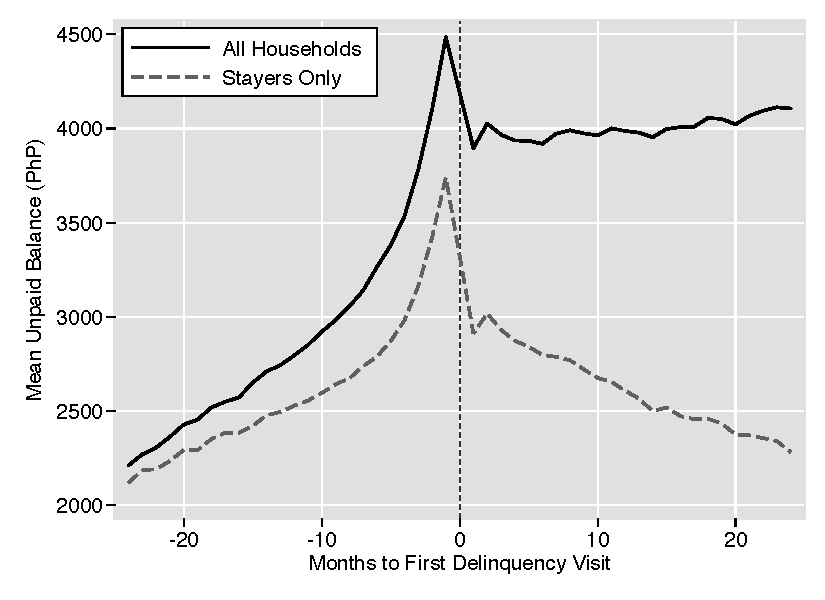
\includegraphics[width=\textwidth,trim={.2cm .2cm .2cm 0cm}, clip=true]{tables/line_bal}
        \label{fig:line_bal}
    \end{subfigure}
    \vskip 1mm \vskip 0pt
    \begin{subfigure}[b]{0.49\textwidth}
        \centering
        \caption[]{\small Days Overdue}
        \vspace{-1mm}
        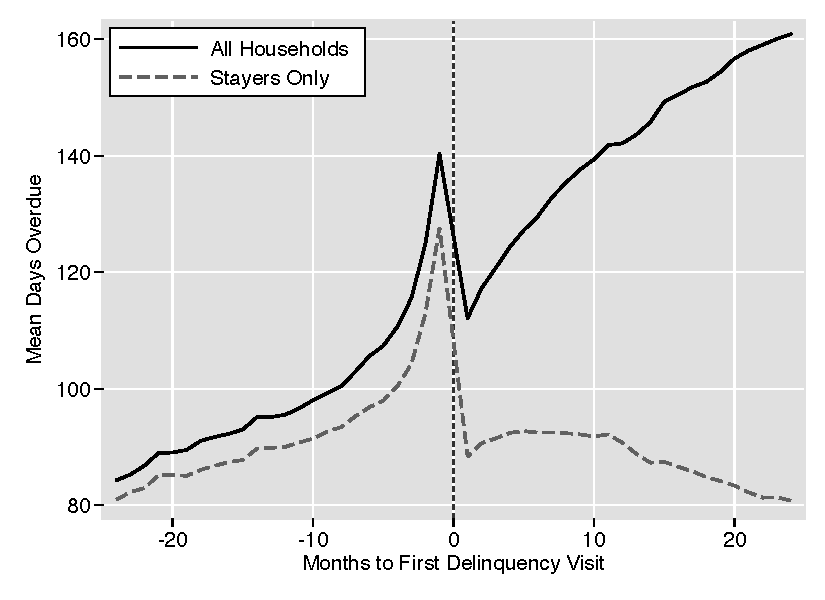
\includegraphics[width=\textwidth,trim={.2cm .2cm .2cm 0cm}, clip=true]{tables/line_ar}
        \label{fig:line_ar}
    \end{subfigure}
    \hfill
    \begin{subfigure}[b]{0.49\textwidth}  
        \centering
        \caption[]{\small Monthly Payment}  
        \vspace{-1mm}
        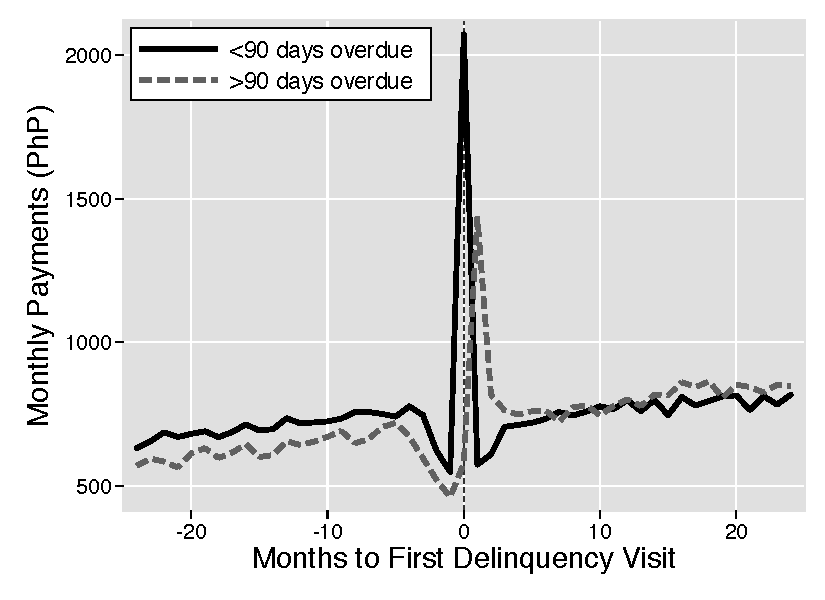
\includegraphics[width=\textwidth,trim={.2cm .2cm .2cm 0cm}, clip=true]{tables/line_pay}
        \label{fig:line_pay}
    \end{subfigure}
    \vskip 1mm \vskip 0pt
    \begin{subfigure}[b]{.49\textwidth}  
        \centering
        \caption[]{\small Average Consumption} 
        \vspace{-1mm}
        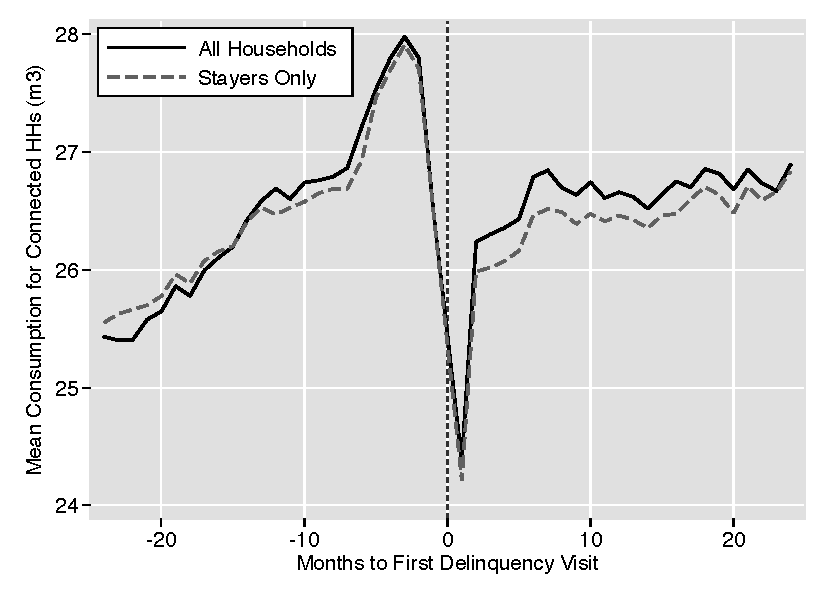
\includegraphics[width=\textwidth,trim={.2cm .2cm .2cm 0cm}, clip=true]{tables/line_c}  
        \label{fig:line_c}
    \end{subfigure}
    \hfill \hspace{.02\textwidth}
    \begin{minipage}{0.47\textwidth}   
    \vspace{-6cm}
    \caption[]
    {\small Mean Outcomes around First Delinquency Visit  \\  \\  Figures include all households with delinquency visits.  Stayers include only households who are connected for the last 6 months of the sample.  Mean monthly payments include zeros when no payment is made. } \label{fig:line_graphs}
    \end{minipage}
\end{figure*} 


To investigate the timing of household responses to delinquency visits, Figure~\ref{fig:line_graphs} plots monthly mean outcomes in months relative to the first delinquency visit for each household.  Outcomes are plotted separately for all households that experience delinquency visits as well as stayer households who experience visits and also remain connected for the last 6 months of the sample.  In the months just preceding a visit, monthly payments (Figure~\ref{fig:line_pay}) decrease suddenly, leading to corresponding increases in unpaid balances (Figure~\ref{fig:line_bal}) and days overdue (Figure~\ref{fig:line_ar}).  Average consumption (Figure~\ref{fig:line_c}) increases slightly as well.  Prior to disconnection, stayers follow similar patterns but with lower levels of delinquency than the population average.

Immediately following the first delinquency visit, monthly payments spike as many households pay their full outstanding balances to prevent any disconnection.  Despite these payments, the average share of households disconnected (Figure~\ref{fig:line_disc}) also spikes to around 24\unskip\% before decreasing, as some households pay for reconnection, and stabilizing at 17\unskip\%, which is likely composed of households who have permanently disconnected.  Stayer households pay more and disconnect less than the population average following a visit.  Disconnection rates for stayers spike to 15\unskip\% before declining to around 4\unskip\% two years later.\footnote{Although stayers are connected for the last 6 months of the sample by definition, disconnection rates do not decline to zero since some stayers experience multiple disconnection spells.}  The decline among stayers accounts for much of the average decline in disconnection rates across the sample.  Although many stayers quickly reconnect within 6 months, reconnections continue accumulating up to one year after a visit.  

This descriptive evidence indicates that many households choose to disconnect for long periods before finally paying for reconnection.  This behavior is consistent with households facing credit-constraints, which prevent them from taking a low-cost loan to fund immediate reconnection.  Instead, households substitute to lower-quality alternative sources of water until they can save enough income for reconnection.  Credit constraints would additionally predict that the most delinquent households at the time of the visit may be the most likely to disconnect following a visit.  The data support this hypothesis, finding that the share disconnected two months after a visit is 32\unskip\% for stayers that are over 90 days delinquent at the time of the visit.  The corresponding share for stayers under 90 days delinquent shrinks to 4\unskip\%.

Another hypothesis may be that households choose to stop paying when they leave their homes for vacation or overseas work.  This mechanism would likely predict a large decrease in water consumption in the months preceding delinquency visits.  Instead, consumption rises consistently between 24 and 2 months before a visit.  Consumption then drops one month before, during, and after a visit, before quickly returning to an average level.  This dip in consumption likely corresponds to connections that are disconnected for less than a month before being reconnected and having their consumption recorded for that month.  Overall, this variation is small given a mean consumption for stayers of 26.7m3 with a standard deviation of 11.1\unskip.  Moreover, delinquency visits are relatively rare, which may make their exact timing difficult for households to predict.  











%The administrative data indicate that 72.5\unskip\% resolve their outstanding balances following a notice.

% At this time, households report paying 

%In practice, the water company often tolerates delinquency well over 60 days, which is consistent with (1) costs of sending and following up on notifications and (2) household demand for credit from the water company.  Households receive notice in 0.66\unskip\% of months.  

% This rate increases to 1.75\unskip\% for households with at least 60 days of delinquency.  

% Figure~\ref{figure:dc_hazard} graphs the probability of receiving a delinquency notice conditional on the level of delinquency for each account.  The water company appears to carefully follow government regulations preventing any disconnection for delinquency below 60 days.  Once households reach 61 days of delinquency, they face some probability of receiving a notice, which triples moving above 90 days unpaid balance.  Conditional on having greater than 90 days of delinquency 




% Appendix on notice!  ( need to get water company confirmation )

%  In practice, the water company tolerates 108.1days of delinquency on average before issuing a notice.  The level of delinquency tolerated before issuing notices also appears uncorrelated with (list measures/demographics...).  ( SHOW REGRESSION IN APPENDIX )  

% Upon receiving a notice of disconnection, connection owners then negotiate for time to pay their outstanding balances.  In 96\unskip\% of notices, owners are agree to pay within 30 days, making an average grace period of 13days according to the water connection survey.  25\unskip\% of connections report having ``enough time'' to make their payments.  

% %The administrative data indicate that 72.5\unskip\% resolve their outstanding balances following a notice.

% Disconnection typically involves workers from the water company placing a metal lock on the water meter stopping the flow.  Once disconnected, connection owners are charged a small, one-time fee of 200 PhP to restore their water service on top of settling any outstanding balances.  The water company is then required to restore service within 48 hours of receiving full payment for reconnection.

% \begin{itemize}
% 	\item No notice: great access to credit, or just not enough time to observe them hitting a
% 	\item Average notice rate!?!

% \end{itemize}

%\footnote{To account for potential mismeasurement in the administrative data, this measure allows connection owners to resolve their outstanding balances within 60 days of receiving notice.}

%In practice, .\unskip\% of owners report receiving advanced notice.  



\section{Model}


\begin{align}\label{eq:u}
E_t \Big[ \sum_{\tau = t}^{t-\tau}  u(w_{\tau},c_{\tau})   \Big]
\end{align}
\begin{align}
c_t + p(w_t) w_t = y_t + A_t - \dfrac{A_{t+1}}{1+r^{a}_{t}}  +  B_t - D_{t+1} \dfrac{B_{t+1}}{1+r^{b}_{t}}  - D_{t+1}
\end{align}
\begin{align}
r^{a}_{t} = 
\begin{cases}
  r_l &\text{ if } A_{t+1} \leq 0  \\
  r_h  &\text{ if } A_{t+1} > 0
\end{cases}
\end{align}
\begin{align}
r^{b}_{t} = 
\begin{cases}
  r_w &\text{ if } A_{t+1} \leq 0 \\
r_h &\text{ if } A_{t+1} > 0 
\end{cases}
\end{align}
\begin{align}
&B_t - D_{t+1} p(w_t) w_t \leq B_{t+1} \leq 0
\end{align}










\section{Model Primitives}




% https://www.cgdev.org/blog/compartamos-context


\cite{karlan2009expanding} find money lenders regularly charge at least 20\% per month for credit.  \cite{gine2014group} offer small monthly loans of 1,000 PhP at 2.5\% monthly interest.

\cite{andreoni2012estimating} estimate rates between 25\% and 35\% in an experimental setting and confirm exponential discounting.  \cite{laibson2007estimating} use a similar consumption-savings structural approach and recover a discount rate of around 15\%.  \cite{gourinchas2002consumption} use a similar structural approach finding a lower discount rate of around 5\%.



%%% Karlan and Zinman

% Informal credit markets
% and serial borrowing from moneylenders charging 20% per month or more is common (e.g., more than
% 30% of our sample reported borrowing from moneylenders during the past year). Trade credit is quite
% uncommon. There are several microlenders operating in Metro Manila, but most MFIs operate on a
% small scale (as noted above) and charge high rates (see below).


\section{Results}

\begin{table}
\centering
\caption{Estimates}\label{table:estimates}
\begin{tabular}{lcc}
& Estimate & Standard Error \\
Interest Rate &0.046&0.00\\
Income Variance &0.300&0.00\\
Water Preference &0.020&0.00\\
\end{tabular} 

\end{table}

\begin{table}
\centering
\caption{Fit}\label{table:fit}
\begin{tabular}{lcc}
& Data & Estimated \\
Mean Usage (m3) &24.9&25.5\\
SD Usage &11.1&2.2\\
Mean Water Debt (PhP) &1232&1222\\
SD Water Debt (PhP) &1281&1821\\
Corr. Usage and Water Debt &0.34&-0.01\\
Mean Usage Pre-Collect (m3) &26.2&25.2\\
Mean Usage Post-Collect &23.4&22.7\\
Diff. (Pre-Post) (m3) &2.8&2.5\\
\end{tabular} 

\end{table}

\begin{figure}
\centering
\caption{Simulated Months}\label{figure:deaton}
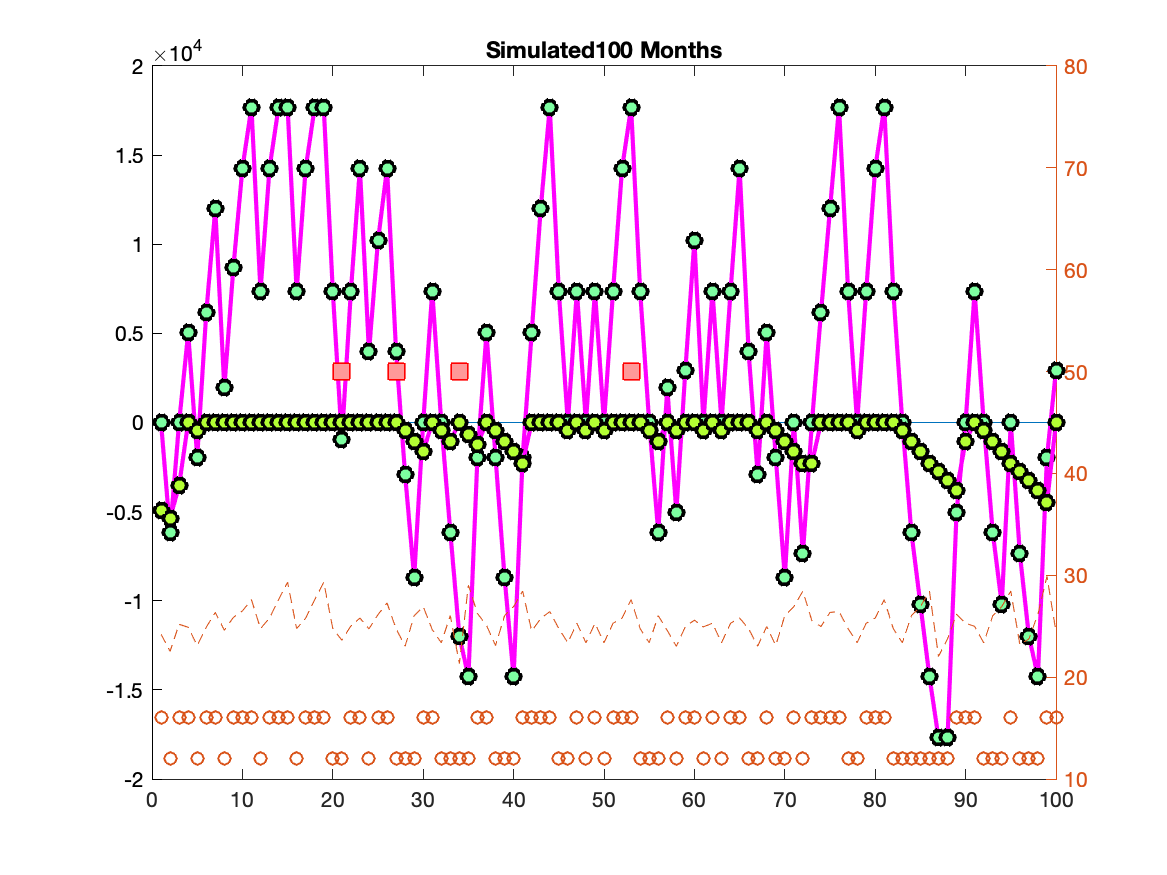
\includegraphics[scale=.5]{tables/deaton.png}
\end{figure}

\begin{table}
\centering
\caption{Counterfactuals}\label{table:counter}
\begin{tabular}{lccc}
& Current & No Water Credit & No Water Credit and \\
&         &                  & Revenue Neutral \\
Water Credit Interest Rate &0.0&1.0&1.0\\
Mean Usage (m3) &25.5&24.2&26.1\\
Compensating Variation  & &51.6&1.4\\
Delinquency Savings  &20.8&20.8&0.0\\
Price Intercept  &16.3&16.3&13.5\\
\end{tabular} 

\end{table}


\section{Appendix}


\begin{table}[h!]
\small
\centering
\caption{ Linear Probability of Receiving a Delinquency Visit }\label{table:tcd_predict}
\vspace{-2mm}
\begin{tabular}{lCCC}
\toprule
& \small (1) & \small (2) & \small (3)  \\
\midrule 
Usage t-1           &  -0.0000316\textsuperscript{a}&  -0.0000347\textsuperscript{a}&  -0.0000555\textsuperscript{a}\\
                    & (0.0000056)                   & (0.0000057)                   & (0.0000087)                   \\[0.5em]
Days Delinquent t-1 &   0.0000554\textsuperscript{a}&   0.0000617\textsuperscript{a}&   0.0000520\textsuperscript{a}\\
                    & (0.0000017)                   & (0.0000018)                   & (0.0000022)                   \\[0.5em]
Unpaid Balance t-1  &   0.0000009\textsuperscript{a}&   0.0000009\textsuperscript{a}&   0.0000013\textsuperscript{a}\\
                    & (0.0000001)                   & (0.0000001)                   & (0.0000001)                   \\[0.5em]
Single House        &  -0.0000600                   &  -0.0000677                   &                               \\
                    & (0.0001986)                   & (0.0002109)                   &                               \\[0.5em]
Apartment           &  -0.0003356\textsuperscript{c}&  -0.0004447\textsuperscript{b}&                               \\
                    & (0.0001820)                   & (0.0001883)                   &                               \\[0.5em]
Age of HoH          &  -0.0000350\textsuperscript{a}&  -0.0000307\textsuperscript{a}&                               \\
                    & (0.0000039)                   & (0.0000039)                   &                               \\[0.5em]
HoH Low Skill Empl. &   0.0004027\textsuperscript{b}&   0.0003920\textsuperscript{b}&                               \\
                    & (0.0001782)                   & (0.0001786)                   &                               \\[0.5em]
HH Size             &   0.0003286\textsuperscript{a}&   0.0003123\textsuperscript{a}&                               \\
                    & (0.0000357)                   & (0.0000356)                   &                               \\[0.5em]
Employed HH Members &  -0.0002616\textsuperscript{a}&  -0.0002750\textsuperscript{a}&                               \\
                    & (0.0000558)                   & (0.0000559)                   &                               \\[0.5em]
Location            &                               &  \checkmark                   &                               \\
Year \tim Month \textsc{FE}&                               &  \checkmark                   &  \checkmark                   \\
Household \textsc{FE}&                               &                               &  \checkmark                   \\
N                   &   1,931,792                   &   1,931,792                   &   1,931,792                   \\
Mean Visits Per Month&      0.0068                   &      0.0068                   &      0.0068                   \\

\bottomrule
\multicolumn{4}{l}{\footnotesize Std. errors clustered at the HH-level. \textsuperscript{c} p$<$0.10,\textsuperscript{b} p$<$0.05,\textsuperscript{a} p$<$0.01 }
\end{tabular}
\end{table}




\begin{table}[h!]
\centering
\caption{Estimating Sample Construction}\label{table:sampleconstruction}
\vspace{-2mm}
\begin{tabular}{l*{1}{cc}}
\toprule
 & Observations & Observations Removed  \\
\midrule
Initial sample   &         798,223  &     \\
Keep residential connections (excluding commercial)   &            &    102,415  \\
Keep connections with payment records &  &   40,708   \\
Keep months with consumption under 200 m3    &            &  73,219     \\
Keep bills $>$ -5,000 PhP and $<$ 80,000 PhP  &  & 116  \\
Keep unpaid bills $>$ -5,000 PhP and $<$ 80,000 PhP &             &     844  \\
Keep payments $>$ -80,000 PhP and $<$ 80,000 PhP    &            &    1   \\
Keep connections with over 30 months of records   &            &   218    \\
Keep connections serving a single household   &            &   721,146    \\
Drop connections that are disconnected for final yr.  &            &   92,459    \\
Final sample & 2,030,876 & \\
\bottomrule
\end{tabular}
\end{table}




\begin{figure}
\centering
\caption{Stayers Share of Households that Receive a Delinquency Visit \\ depending on Days Delinquent in the Previous Month}\label{figure:dc_hazardstayers}
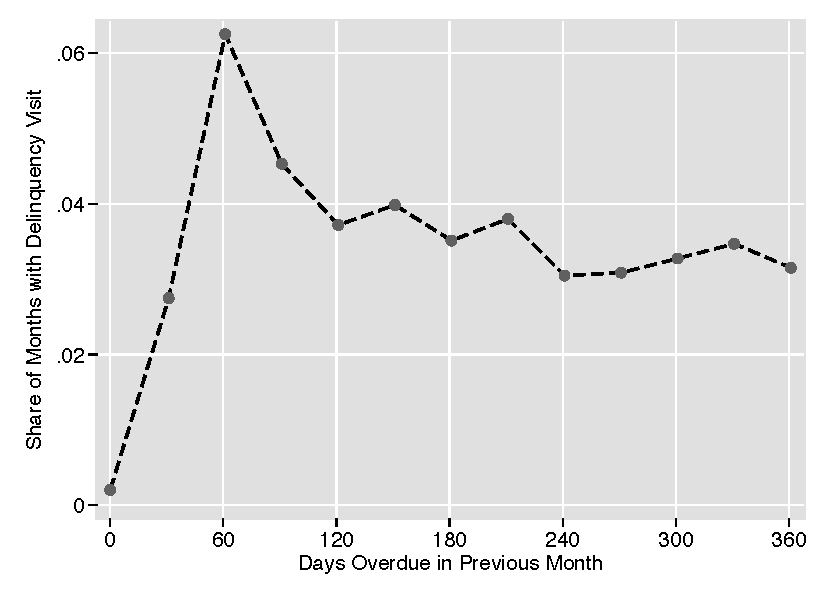
\includegraphics[scale=.7]{tables/connected_visit_hazard.pdf} \\
{ \footnotesize Only stayer households. }
\end{figure}


\begin{table}[h!]
\centering
\caption{Descriptives for Stayers}\label{table:descriptives_stayers}
\vspace{-2mm}
\begin{tabular}{l*{1}{cccccc}}
\toprule
 & Mean & SD & Min & 25th & 75th & Max  \\
\midrule
 Usage (m3)  & 30.0  & 20.5  & 0.0  & 17.0  & 38.0  & 200.0  \\ 
 Bill  & 931  & 1,269  & -4,862  & 323  & 1,122  & 78,409  \\ 
 Unpaid Balance  & 3,009  & 5,953  & -4,995  & 330  & 3,016  & 79,959  \\ 
 Share of Months with Payment  & 0.62  & 0.49  & 0.00  & 0.00  & 1.00  & 1.00  \\ 
 Payment Size  & 1,448  & 1,769  & 0  & 500  & 1,753  & 76,029  \\ 
 Days Delinquent  & 90.9  & 161.8  & 0.0  & 0.0  & 91.0  & 720.0  \\ 
 Delinquency Visits per HH  & 1.35  & 0.63  & 1.00  & 1.00  & 2.00  & 6.00  \\ 
 Share of Months Disconnected  & 0.04  & 0.19  & 0.00  & 0.00  & 0.00  & 1.00  \\ 

\bottomrule
\multicolumn{7}{c}{Total Households: 11,856  Obs. per Household: 61.8 Total Obs.: 731,935}
\end{tabular}
\end{table}


\nocite{*}
\singlespacing
\setlength{\bibsep}{7pt}
\bibliographystyle{abbrvnat}
\bibliography{ref}





\end{document}


